\chapter{Технологический раздел}
В данном разделе рассматриваются различные СУБД реляционных баз данных, проводится их сравнение по выделенным критериям, представлены  средства реализации программного обеспечения, демонстрируется процесс создания таблиц, функций, триггеров и ролей базы данных. Демонстрируется работа программного обеспечения.

\section{Выбор СУБД}
Наиболее распространенными СУБД реляционных баз данных являются:
\begin{itemize}
    \item[---] PostgreSQL~\cite{Psql};
    \item[---] MySQL~\cite{MySQL};
    \item[---] Microsoft SQL Server~\cite{MSSQL};
    \item[---] Oracle DB~\cite{Oracle}.
\end{itemize}

Выделим критерии для сравнения приведенных СУБД:
\begin{itemize}
    \item[---] КР1 --- бесплатное распространение;
    \item[---] КР2 --- поддержка ролевой модели;
    \item[---] КР3 --- производительность~\cite{ismail2019oracle, solarz2020oracle};
\end{itemize}

В таблице~\ref{tbl:versus_subd} приводится сравнение рассматриваемых СУБД, по выделенным критериям.

\begin{table}[H]
    \begin{center}
        \caption{Сравнение СУБД}
        \begin{tabular}{|c|c|c|c|c|}
            \hline
            \textbf{Решение} & \textbf{КР1} & \textbf{КР2} & \textbf{КР3} \\
            \hline
            PostgreSQL & + & + & 1 \\
            \hline
            MySQL & + & + & 4 \\
            \hline
            Microsoft SQL Server & - & + & 3 \\
            \hline
            Oracle DB & - & + & 2 \\
            \hline
        \end{tabular}
        \label{tbl:versus_subd}
    \end{center}
\end{table}

По результатам сравнения в качестве используемой СУБД был выбран PostgreSQL, так как он удовлетворяет всем поставленным критериям и является наиболее быстрым из всех.

\section{Выбор средств реализации ПО}

В качестве языка программирования был выбран Kotlin~\cite{Kotlin}, поскольку разработка ориентирована на мобильные устройства, большинство которых функционирует под управлением Android~\cite{Android_stat}. Для работы с базой данных был выбран фреймворк Exposed~\cite{Exposed}, который позволяет использовать DSL для описания запросов, а также поддерживает объектно-ориентированный подход к доступу данным. Для реализации серверной части был выбран фреймфорк Ktor~\cite{Ktor}. Для написания клиентского приложения и интерфейса пользователя был использован фреймворк Jetpack Compose~\cite{Compose}.

\section{Архитектура приложения}
Для реализации приложения был выбран подход MVVM (Model-View-ViewModel)~\cite{MVVM}. В нём приложение разделяется на три слоя:

\begin{itemize}
	\item[---] Model отвечает за бизнес-логику и доступ к данным;
	\item[---] View представляет собой пользовательский интерфейс и отвечает только за отображение данных;
	\item[---] ViewModel выступает в качестве посредника между Model и View, обрабатывая пользовательские события, управляя состоянием интерфейса и предоставляя данные в удобной для отображения форме.
\end{itemize}

\section{Создание таблиц базы данных}

В листингах~\ref{lst:book} ---~\ref{lst:queue} представлено создание таблиц и описание соответствующих ограничений к нииммм.

\begin{center}
	\captionsetup{justification=raggedright,singlelinecheck=off}
	\begin{lstlisting}[language=sql, frame=single, numbers=left, label=lst:book, caption=Создание таблицы book]
CREATE TABLE IF NOT EXISTS book (
	id UUID PRIMARY KEY,
	title VARCHAR(255) NOT NULL,
	annotation TEXT,
	publisher_id UUID REFERENCES publisher(id) ON DELETE CASCADE,
	publication_year INT,
	ISBN VARCHAR(50),
	bbk_id UUID REFERENCES bbk(id) ON DELETE RESTRICT NOT NULL,
	media_type VARCHAR(100),
	volume TEXT,
	language VARCHAR(100),
	original_language VARCHAR(100),
	copies INT DEFAULT 0 NOT NULL,
	available_copies INT DEFAULT 0 NOT NULL CHECK (available_copies <= copies)
);
	\end{lstlisting}
\end{center}

\begin{center}
	\captionsetup{justification=raggedright,singlelinecheck=off}
	\begin{lstlisting}[language=sql, frame=single, numbers=left, caption=Создание таблицы author]
CREATE TABLE IF NOT EXISTS author (
	id UUID PRIMARY KEY,
	name VARCHAR(255) NOT NULL
);
	\end{lstlisting}
\end{center}

\begin{center}
	\captionsetup{justification=raggedright,singlelinecheck=off}
	\begin{lstlisting}[language=sql, frame=single, numbers=left, caption=Создание таблицы связки book\_author]
CREATE TABLE IF NOT EXISTS book_author (
	book_id UUID REFERENCES book(id) ON DELETE CASCADE,
	author_id UUID REFERENCES author(id) ON DELETE CASCADE,
	PRIMARY KEY (book_id, author_id)
);
	\end{lstlisting}
\end{center}

\begin{center}
	\captionsetup{justification=raggedright,singlelinecheck=off}
	\begin{lstlisting}[language=sql, frame=single, numbers=left, caption=Создание таблицы publisher]
CREATE TABLE IF NOT EXISTS publisher (
	id UUID PRIMARY KEY,
	name VARCHAR(255) NOT NULL,
	description VARCHAR(255),
	email VARCHAR(50),
	phone_number VARCHAR(20)
);
	\end{lstlisting}
\end{center}

\begin{center}
	\captionsetup{justification=raggedright,singlelinecheck=off}
	\begin{lstlisting}[language=sql, frame=single, numbers=left, caption=Создание таблицы bbk]
CREATE TABLE IF NOT EXISTS bbk (
	id UUID PRIMARY KEY,
	code VARCHAR(16) NOT NULL,
	description VARCHAR(255) NOT NULL
);	
	\end{lstlisting}
\end{center}

\begin{center}
	\captionsetup{justification=raggedright,singlelinecheck=off}
	\begin{lstlisting}[language=sql, frame=single, numbers=left, caption=Создание таблицы apu]
CREATE TABLE IF NOT EXISTS apu (
	id UUID PRIMARY KEY,
	term VARCHAR(100) NOT NULL,
	bbk_id UUID REFERENCES bbk(id) ON DELETE CASCADE NOT NULL
);
	\end{lstlisting}
\end{center}

\begin{center}
	\captionsetup{justification=raggedright,singlelinecheck=off}
	\begin{lstlisting}[language=sql, frame=single, numbers=left, caption=Создание таблицы user]
CREATE TABLE IF NOT EXISTS "user" (
	id UUID PRIMARY KEY,
	name VARCHAR(50) NOT NULL,
	surname VARCHAR(50) NOT NULL,
	second_name VARCHAR(50),
	email VARCHAR(50),
	password VARCHAR(100) NOT NULL,
	phone_number VARCHAR(20) NOT NULL,
	role VARCHAR(20) DEFAULT 'READER' NOT NULL
);
	\end{lstlisting}
\end{center}

\begin{center}
	\captionsetup{justification=raggedright,singlelinecheck=off}
	\begin{lstlisting}[language=sql, frame=single, numbers=left, caption=Создание таблицы issuance]
CREATE TABLE IF NOT EXISTS issuance (
	id UUID PRIMARY KEY,
	book_id UUID REFERENCES book(id) ON DELETE CASCADE NOT NULL,
	user_id UUID REFERENCES "user"(id) ON DELETE CASCADE NOT NULL,
	issuance_date DATE NOT NULL,
	return_date DATE NOT NULL CHECK (return_date > issuance_date)
);
	\end{lstlisting}
\end{center}

\begin{center}
	\captionsetup{justification=raggedright,singlelinecheck=off}
	\begin{lstlisting}[language=sql, frame=single, numbers=left, caption=Создание таблицы reservation]
CREATE TABLE IF NOT EXISTS reservation (
	id UUID PRIMARY KEY,
	book_id UUID REFERENCES book(id) ON DELETE CASCADE NOT NULL,
	user_id UUID REFERENCES "user"(id) ON DELETE CASCADE NOT NULL,
	reservation_date DATE NOT NULL,
	cancel_date DATE NOT NULL CHECK (cancel_date > reservation_date)
);
	\end{lstlisting}
\end{center}

\begin{center}
	\captionsetup{justification=raggedright,singlelinecheck=off}
	\begin{lstlisting}[language=sql, frame=single, numbers=left, caption=Создание таблицы favorite]
CREATE TABLE IF NOT EXISTS user_book (
	user_id UUID REFERENCES "user"(id) ON DELETE CASCADE,
	book_id UUID REFERENCES book(id) ON DELETE CASCADE,
	PRIMARY KEY (user_id, book_id)
);
	\end{lstlisting}
\end{center}

\begin{center}
	\captionsetup{justification=raggedright,singlelinecheck=off}
	\begin{lstlisting}[language=sql, frame=single, numbers=left, label=lst:queue, caption=Создание таблицы queue]
CREATE TABLE IF NOT EXISTS queue (
	id UUID PRIMARY KEY,
	book_id UUID REFERENCES book(id) ON DELETE CASCADE NOT NULL,
	user_id UUID REFERENCES "user"(id) ON DELETE CASCADE NOT NULL,
	created_at TIMESTAMP NOT NULL DEFAULT NOW()
);
	\end{lstlisting}
\end{center}

\section{Создание функций базы данных}
В листингах~\ref{lst:func_1} ---~\ref{lst:func_3} представлено создание функций базы данных рассмотренных в конструкторском разделе.

Функции process\_book\_return и process\_book\_loan предполагается вызывать из триггеров, поэтому они объявлены как триггерные функции~\cite{триггерная_функция}.

\begin{center}
	\captionsetup{justification=raggedright,singlelinecheck=off}
	\begin{lstlisting}[language=sql, frame=single, numbers=left, label=lst:func_1, caption=Создание функции process\_book\_return]
CREATE OR REPLACE FUNCTION process_book_return()
RETURNS TRIGGER 
LANGUAGE plpgsql
AS $$
DECLARE
	next_user uuid;
	book_uuid uuid;
	total_copies int;
	free_copies int;
BEGIN
	book_uuid := OLD.book_id;
	
	SELECT copies, available_copies
	INTO total_copies, free_copies
	FROM book
	WHERE id = book_uuid;
	
	IF free_copies < total_copies THEN
		UPDATE book
		SET available_copies = available_copies + 1
		WHERE id = book_uuid;
	END IF;
	
	SELECT user_id INTO next_user
	FROM queue
	WHERE book_id = book_uuid
	ORDER BY created_at
	LIMIT 1;
	
	IF next_user IS NOT NULL THEN
		INSERT INTO reservation(id, book_id, user_id, reservation_date, cancel_date)
		VALUES (gen_random_uuid(), book_uuid, next_user, NOW(), NOW() + INTERVAL '3 days');
		
		DELETE FROM queue
		WHERE user_id = next_user AND book_id = book_uuid;
	END IF;
	
	RETURN OLD;
END;
$$;

	\end{lstlisting}
\end{center}

\begin{center}
	\captionsetup{justification=raggedright,singlelinecheck=off}
	\begin{lstlisting}[language=sql, frame=single, numbers=left, label=lst:func_2, caption=Создание функции process\_book\_loan]
CREATE OR REPLACE FUNCTION process_book_loan()
RETURNS TRIGGER
LANGUAGE plpgsql
AS $$
DECLARE
	available integer;
BEGIN
	SELECT available_copies
	INTO available
	FROM book
	WHERE id = NEW.book_id
	FOR UPDATE;
	
	IF available <= 0 THEN
		RAISE EXCEPTION 'Нет доступных экземпляров книги с id=%', NEW.book_id;
	END IF;
	
	UPDATE book
	SET available_copies = available_copies - 1
	WHERE id = NEW.book_id;
	
	RETURN NEW;
END;
$$;

	\end{lstlisting}
\end{center}


\begin{center}
	\captionsetup{justification=raggedright,singlelinecheck=off}
	\begin{lstlisting}[language=sql, frame=single, numbers=left, label=lst:func_3, caption=Создание функции get\_queue\_number]
CREATE OR REPLACE FUNCTION get_queue_number(p_book_id UUID, p_user_id UUID)
RETURNS INT 
LANGUAGE plpgsql
AS $$
BEGIN
	RETURN (
		SELECT position
		FROM (
			SELECT user_id,
				ROW_NUMBER() OVER (PARTITION BY book_id ORDER BY created_at) AS position
			FROM queue
			WHERE book_id = p_book_id
		) q
		WHERE q.user_id = p_user_id
	);
END;
$$;

	\end{lstlisting}
\end{center}

\section{Создание триггеров базы данных}
В листингах~\ref{lst:tr_1} ---~\ref{lst:tr_2} представлено создание триггеров базы данных.

\begin{center}
	\captionsetup{justification=raggedright,singlelinecheck=off}
	\begin{lstlisting}[language=sql, frame=single, numbers=left, label=lst:tr_1, caption=Создание тригеров для таблицы reservation]
CREATE TRIGGER trg_return_book_from_reservation
AFTER DELETE ON reservation
FOR EACH ROW
EXECUTE FUNCTION process_book_return();
		
CREATE TRIGGER trg_loan_book_to_reservation
BEFORE INSERT ON reservation
FOR EACH ROW
EXECUTE FUNCTION process_book_loan();
	\end{lstlisting}
\end{center}

\begin{center}
	\captionsetup{justification=raggedright,singlelinecheck=off}
	\begin{lstlisting}[language=sql, frame=single, numbers=left, label=lst:tr_2, caption=Создание тригеров для таблицы issuance]
CREATE TRIGGER trg_return_book_from_reservation
AFTER DELETE ON issuance
FOR EACH ROW
EXECUTE FUNCTION process_book_return();

CREATE TRIGGER trg_loan_book_to_reservation
BEFORE INSERT ON issuance
FOR EACH ROW
EXECUTE FUNCTION process_book_loan();
	\end{lstlisting}
\end{center}

\section{Создание ролей базы данных}
В листингах~\ref{lst:guest} ---~\ref{lst:moderator} представлено создание ролей базы данных и выдача соответствующих прав каждой из них.

\begin{center}
	\captionsetup{justification=raggedright,singlelinecheck=off}
	\begin{lstlisting}[language=sql, frame=single, numbers=left, label=lst:guest, caption=Создание роли гостя]
CREATE ROLE guest
	NOSUPERUSER
	NOCREATEDB
	NOCREATEROLE
	NOINHERIT
	NOREPLICATION
	NOBYPASSRLS
	LOGIN
	PASSWORD 'guest';
	
GRANT SELECT ON book, author, bbk, apu, book_author TO guest;
GRANT SELECT (id, name) ON publisher TO guest;
GRANT SELECT, INSERT ON "user" TO guest;
	\end{lstlisting}
\end{center}

\begin{center}
	\captionsetup{justification=raggedright,singlelinecheck=off}
	\begin{lstlisting}[language=sql, frame=single, numbers=left, caption=Создание роли читателя]
CREATE ROLE reader
	NOSUPERUSER
	NOCREATEDB
	NOCREATEROLE
	NOINHERIT
	NOREPLICATION
	NOBYPASSRLS
	LOGIN
	PASSWORD 'reader';
	
	GRANT SELECT ON book, author, bbk, apu, book_author TO reader;
	GRANT SELECT (id, name) ON publisher TO reader;
	GRANT SELECT, UPDATE ON "user" TO reader;
	GRANT SELECT ON favorite, queue, issuance, reservation TO reader;
	GRANT INSERT, DELETE ON favorite, reservation, queue TO reader;
	\end{lstlisting}
\end{center}

\begin{center}
	\captionsetup{justification=raggedright,singlelinecheck=off}
	\begin{lstlisting}[language=sql, frame=single, numbers=left, caption=Создание роли библиотекаря]
CREATE ROLE librarian
	NOSUPERUSER
	NOCREATEDB
	NOCREATEROLE
	NOINHERIT
	NOREPLICATION
	NOBYPASSRLS
	LOGIN
	PASSWORD 'librarian';

GRANT SELECT ON book, author, bbk, apu, book_author, publisher TO librarian;
GRANT SELECT, DELETE ON reservation TO librarian;
GRANT SELECT, INSERT, DELETE ON issuance TO librarian;
	\end{lstlisting}
\end{center}

\begin{center}
	\captionsetup{justification=raggedright,singlelinecheck=off}
	\begin{lstlisting}[language=sql, frame=single, numbers=left, label=lst:moderator, caption=Создание роли модератора]
CREATE ROLE moderator
	SUPERUSER
	CREATEDB
	CREATEROLE
	INHERIT
	REPLICATION
	BYPASSRLS
	LOGIN
	PASSWORD 'moderator';
	\end{lstlisting}
\end{center}

\section{Демонстрация работы программы}

На рисунках~\ref{fig:home} ---~\ref{fig:moderator} изображены экраны приложения, на которых демонстрируется функционал читателя, библиотекаря, модератора.

\begin{figure}[H]
	\centering
	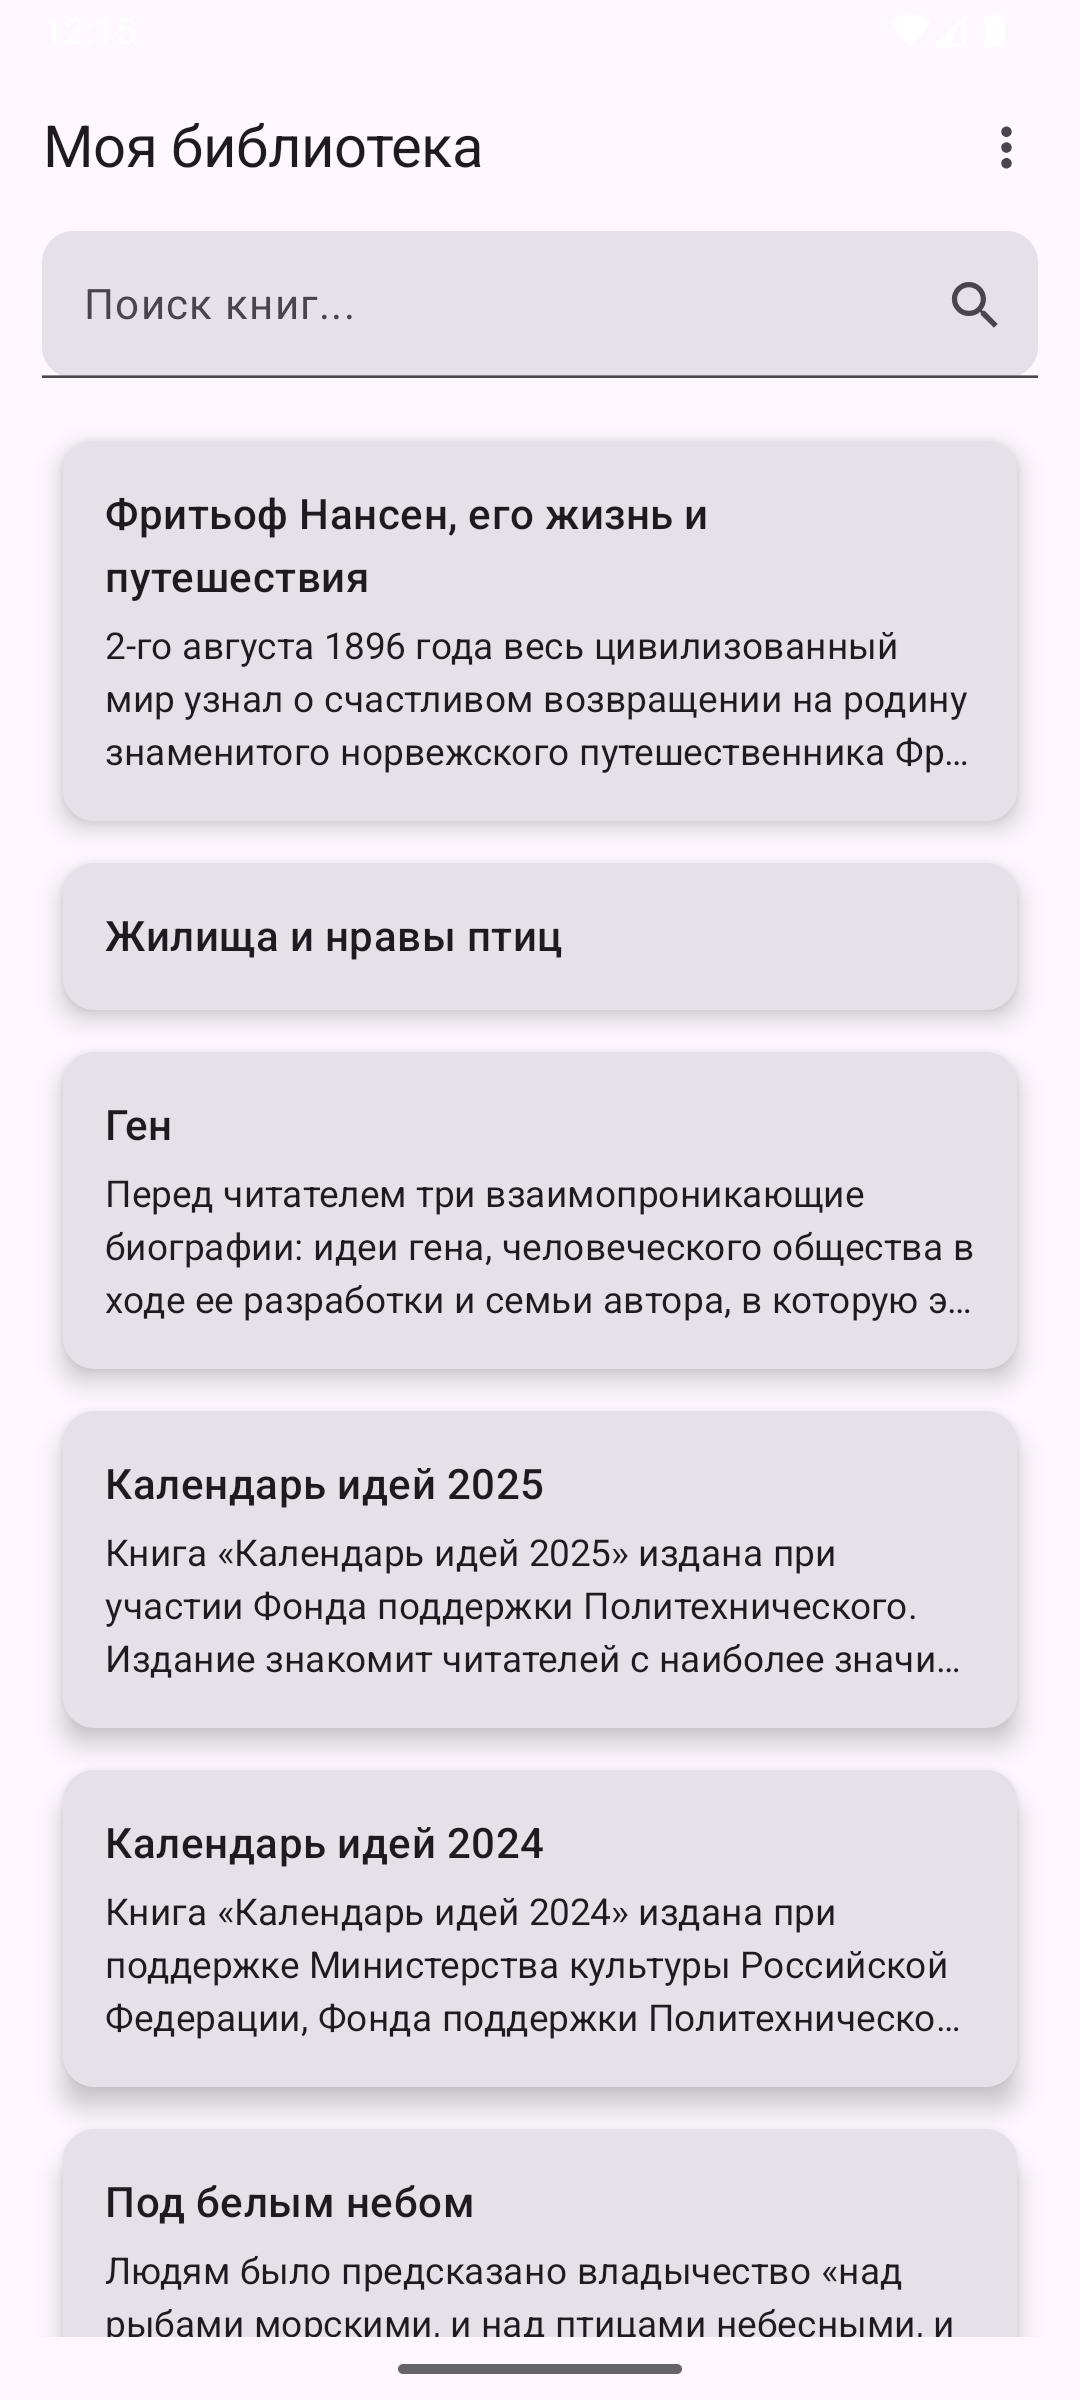
\includegraphics[scale=0.15]{img/home.png}
	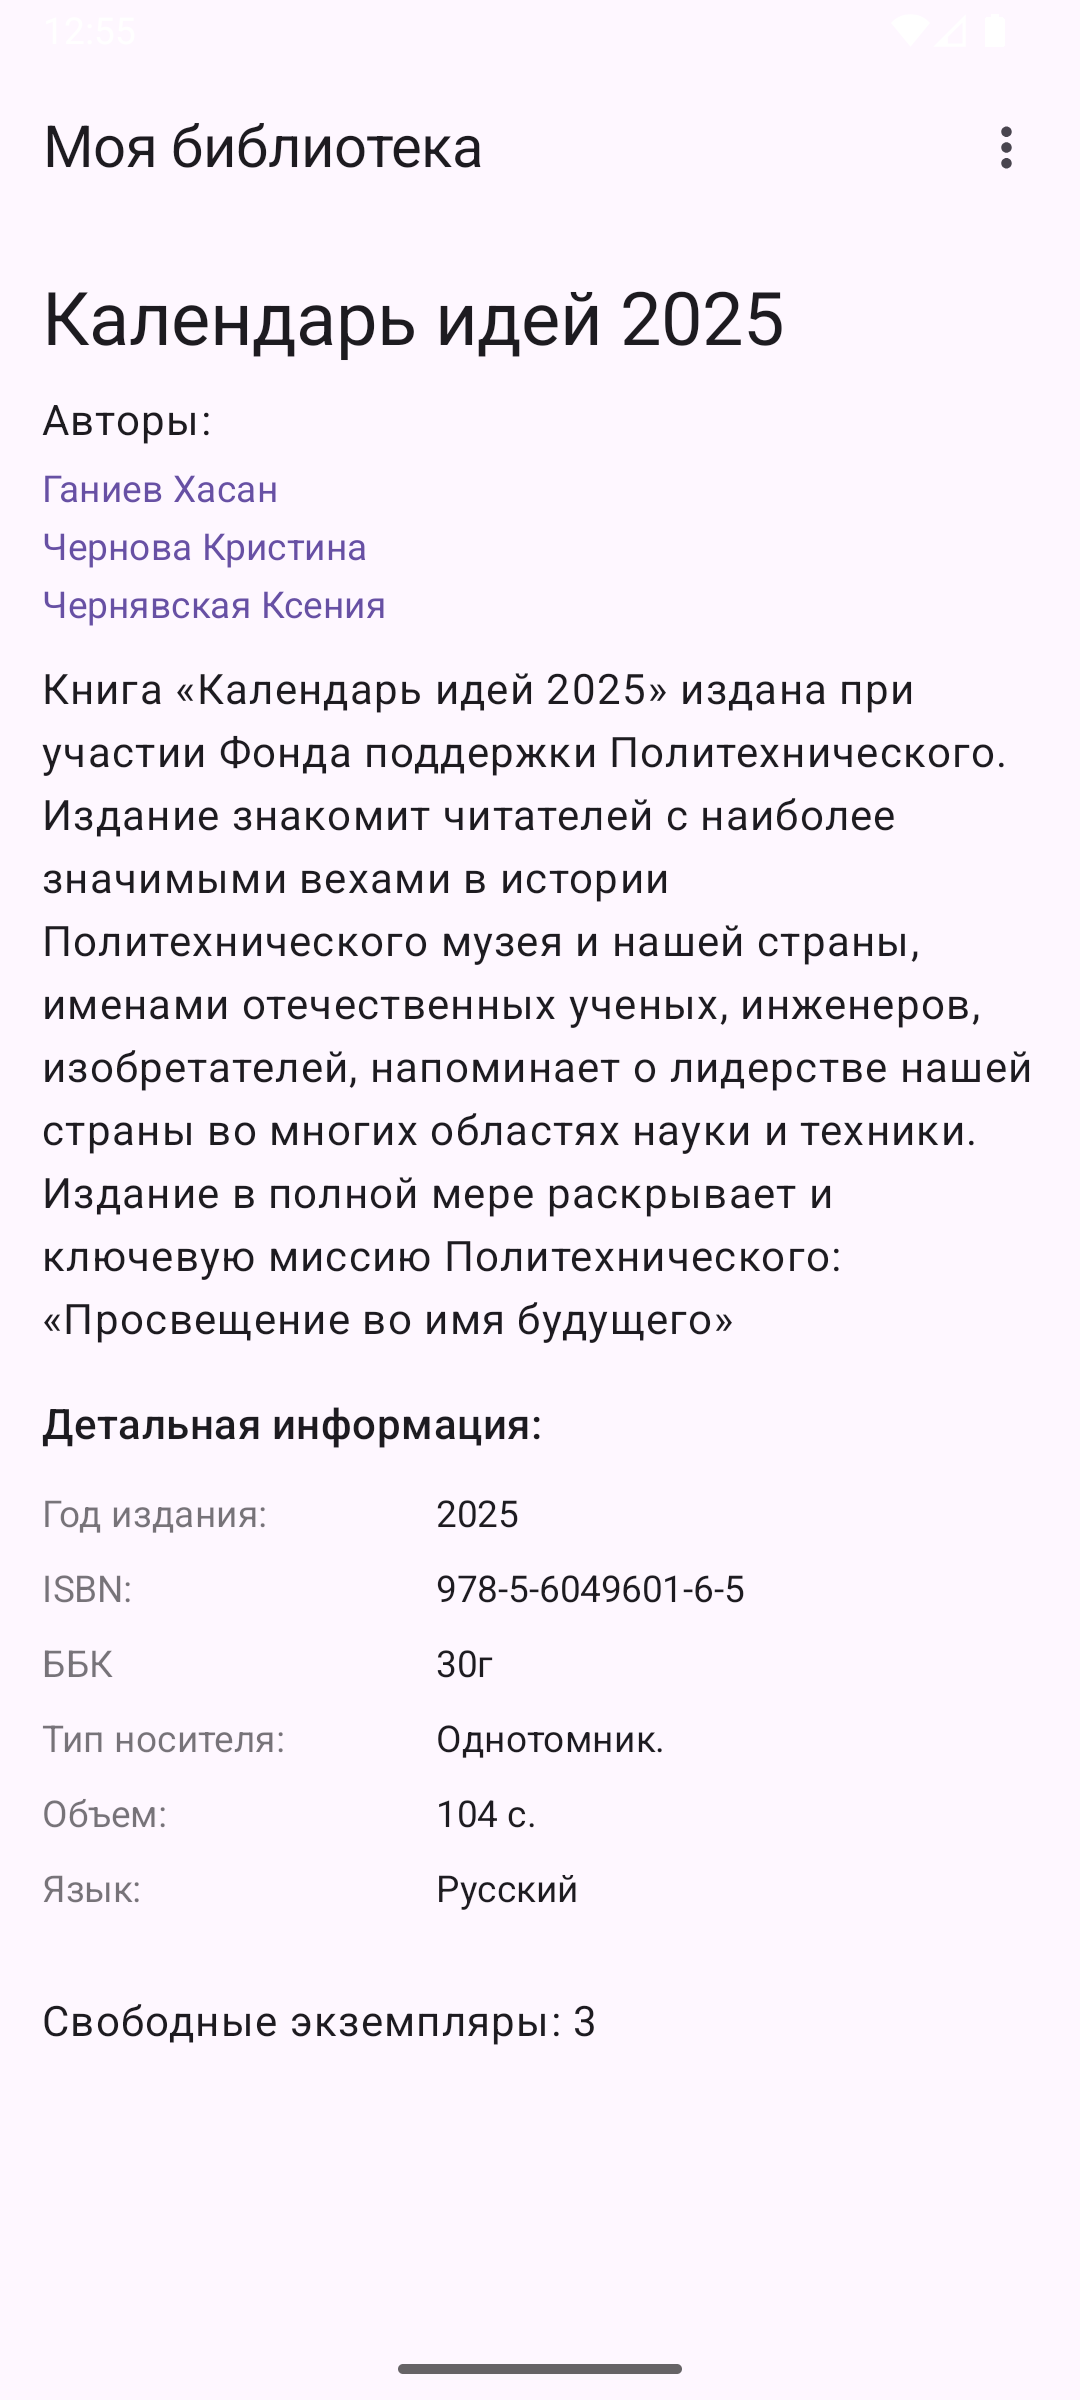
\includegraphics[scale=0.15]{img/book_detail.png}
	\caption{Домашний экран приложения}
	\label{fig:home}
\end{figure}

\begin{figure}[H]
	\centering
	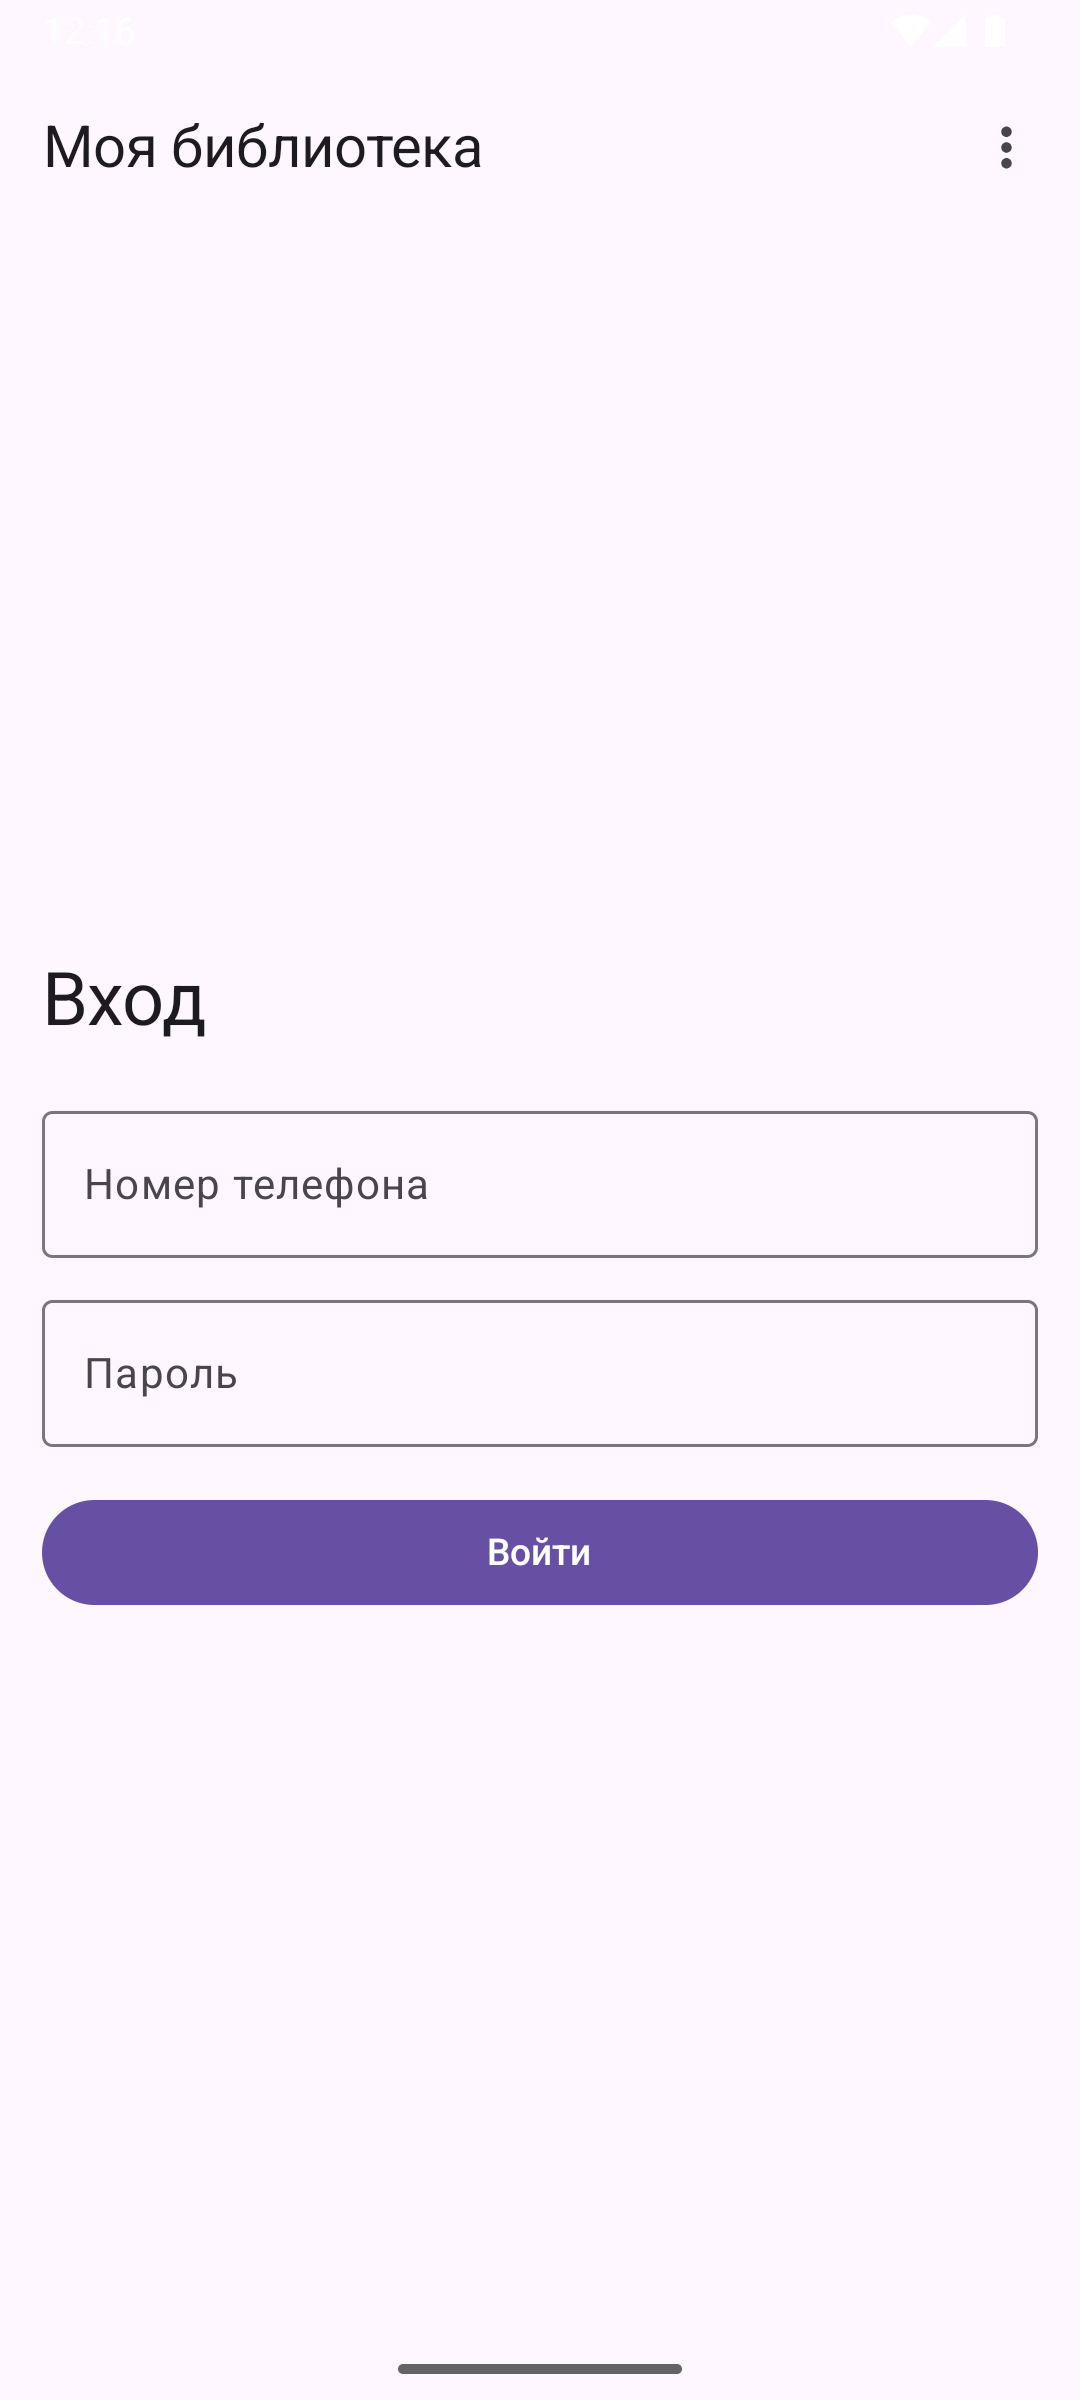
\includegraphics[scale=0.125]{img/login.png}
	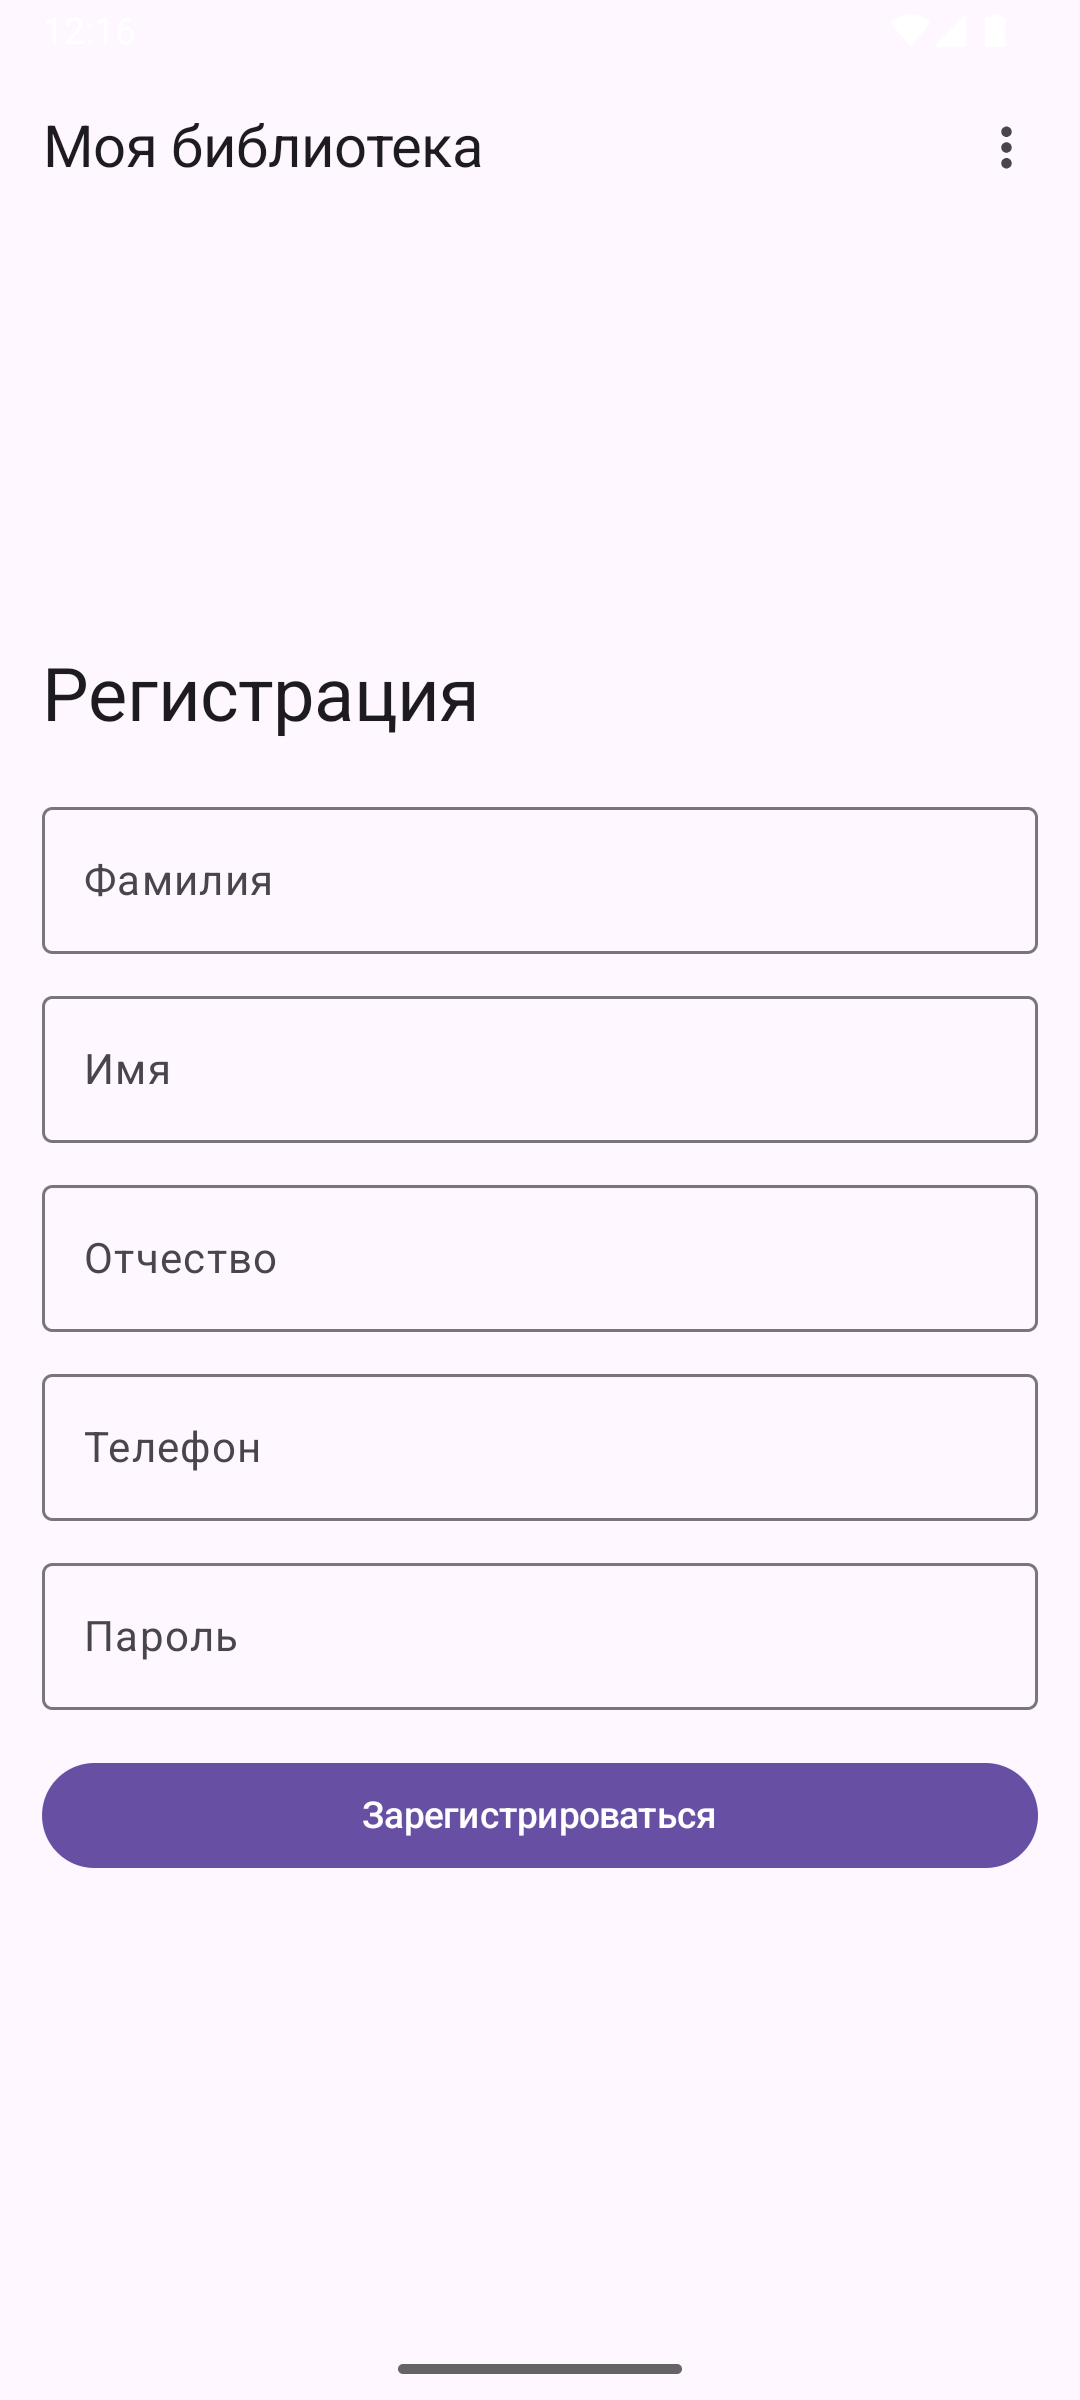
\includegraphics[scale=0.125]{img/register.png}
	\caption{Экраны авторизации и регистрации}
\end{figure}

\begin{figure}[H]
	\centering
	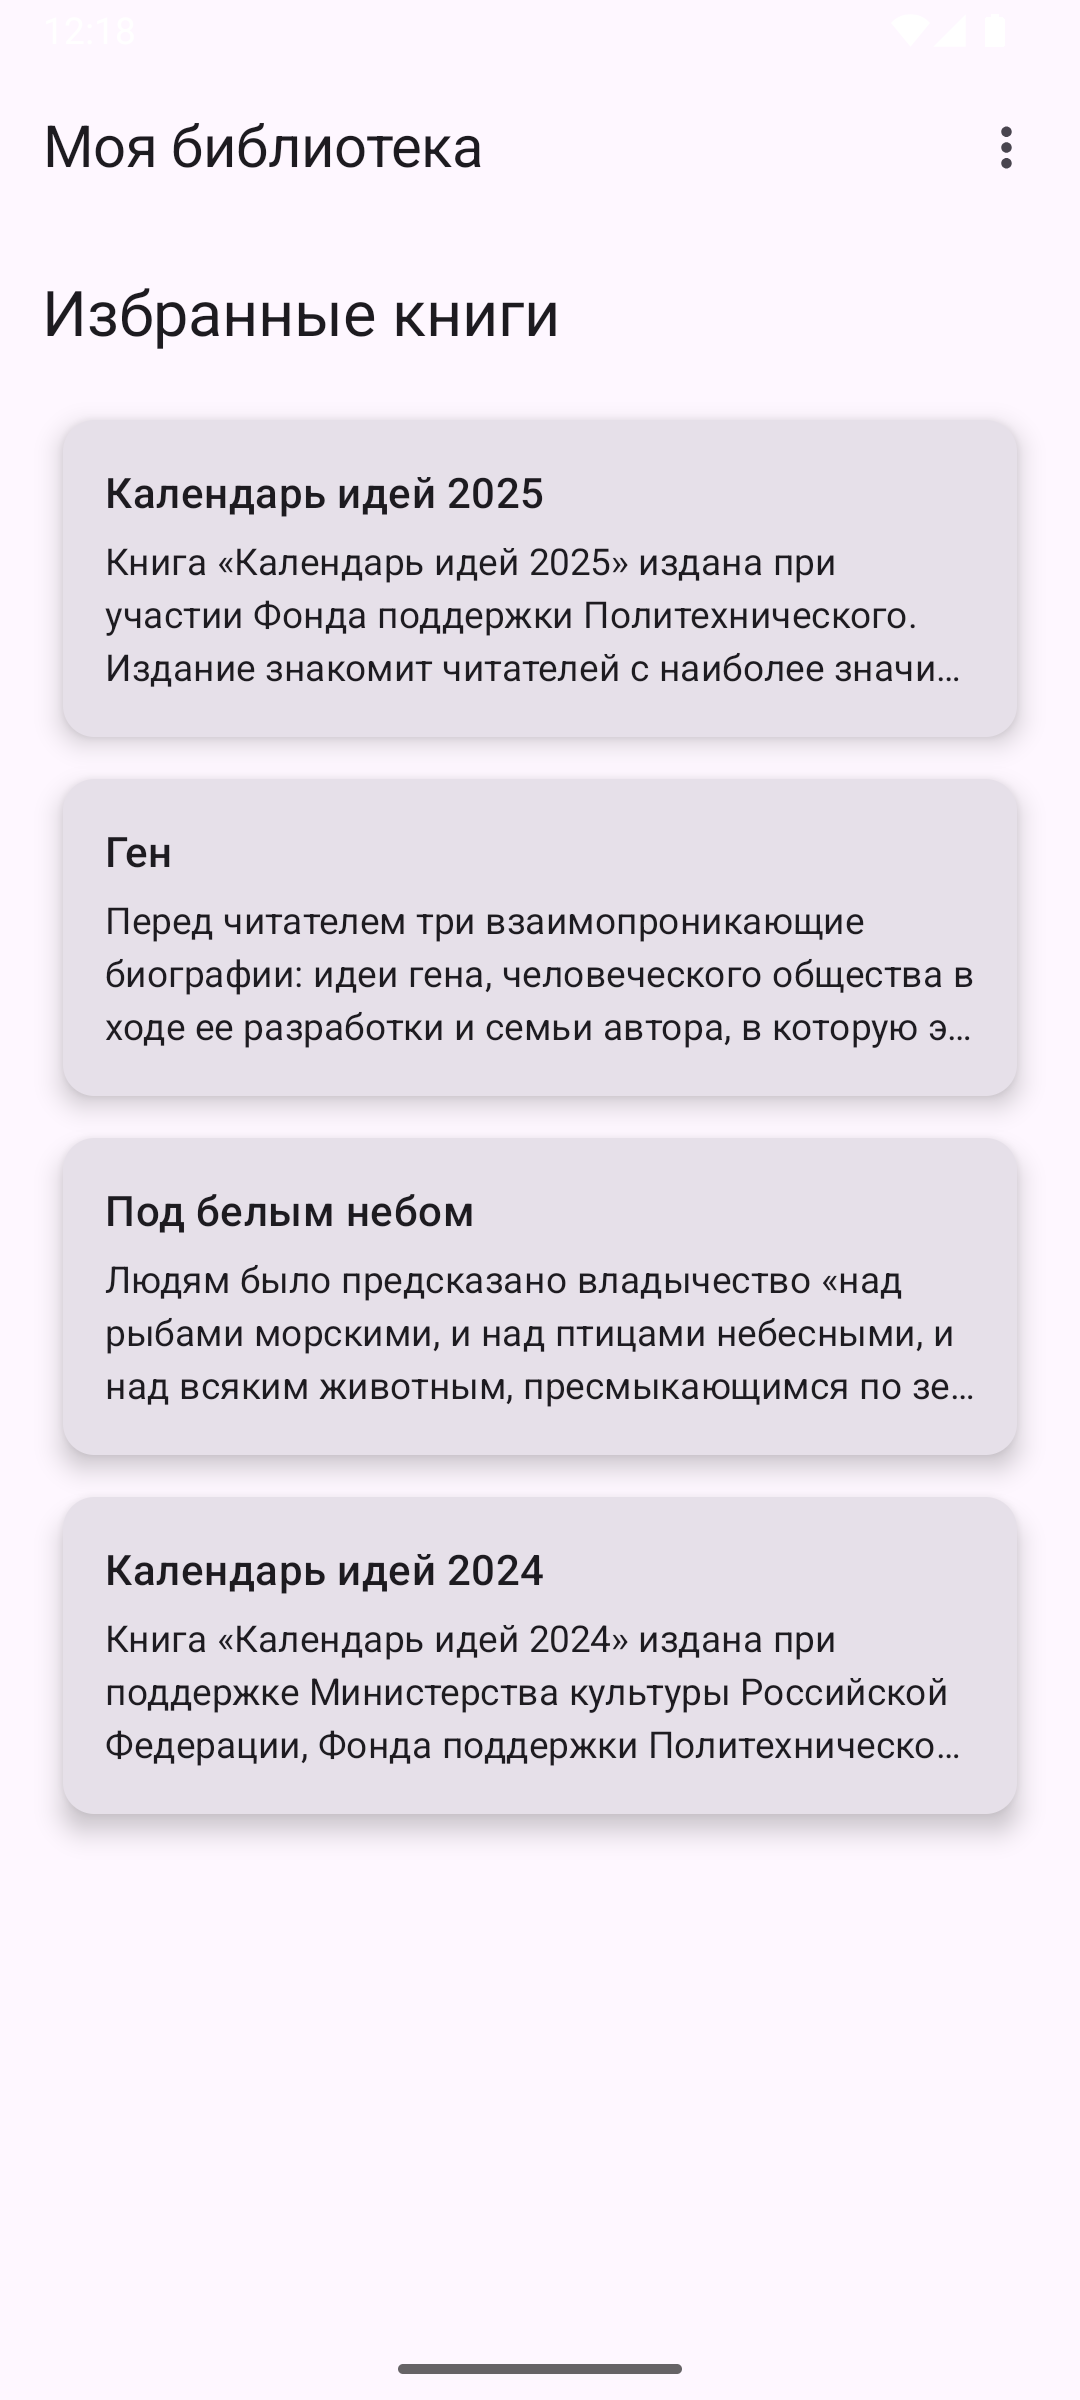
\includegraphics[scale=0.125]{img/favorite.png}
	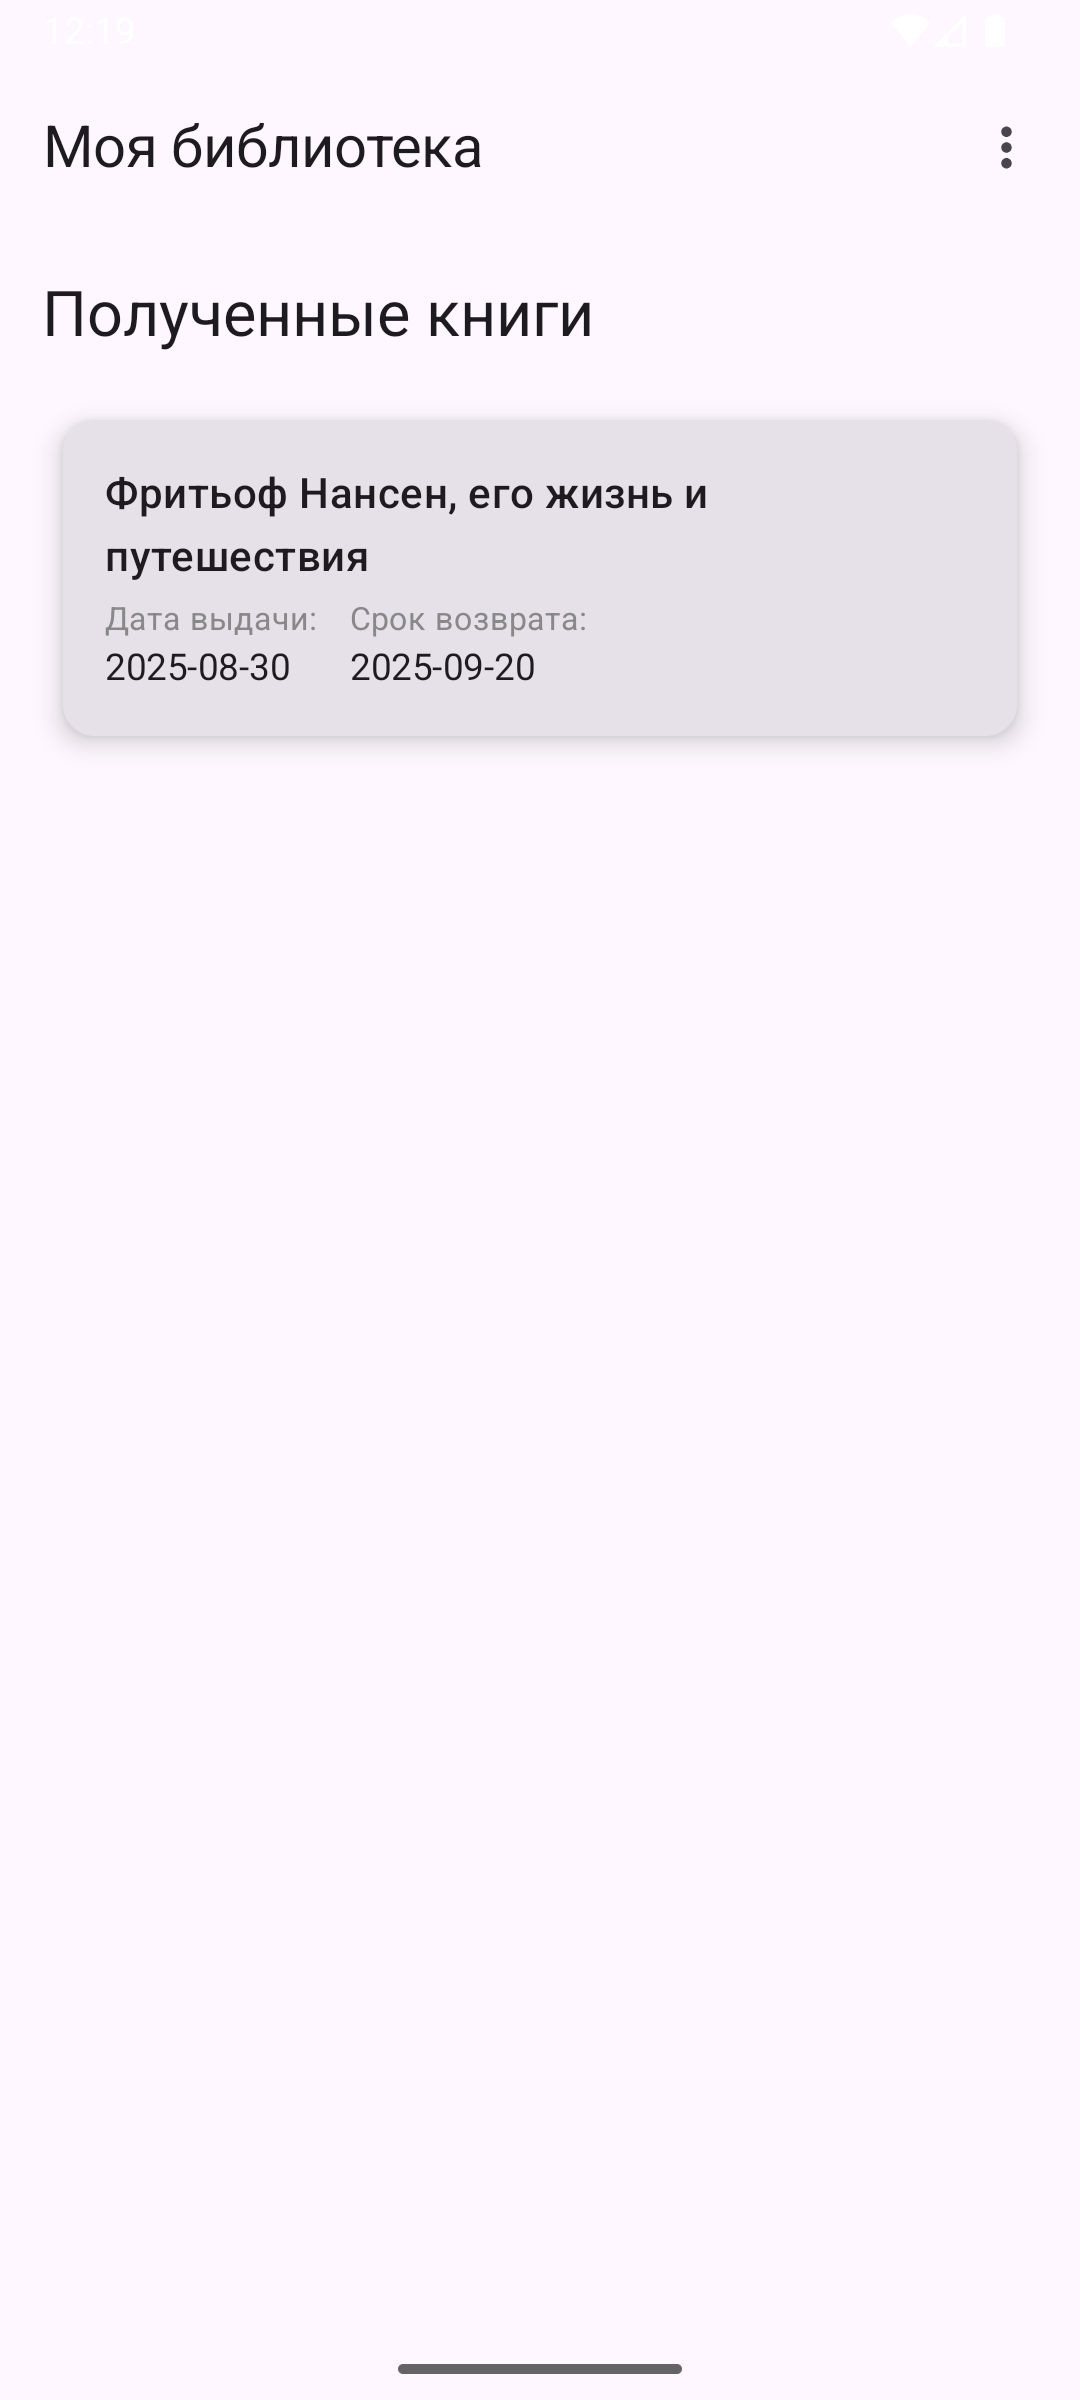
\includegraphics[scale=0.125]{img/issuance.png}
	
\includegraphics[scale=0.125]{img/queue.png}
	\caption{Экраны читателя}
\end{figure}

\begin{figure}[H]
	\centering
	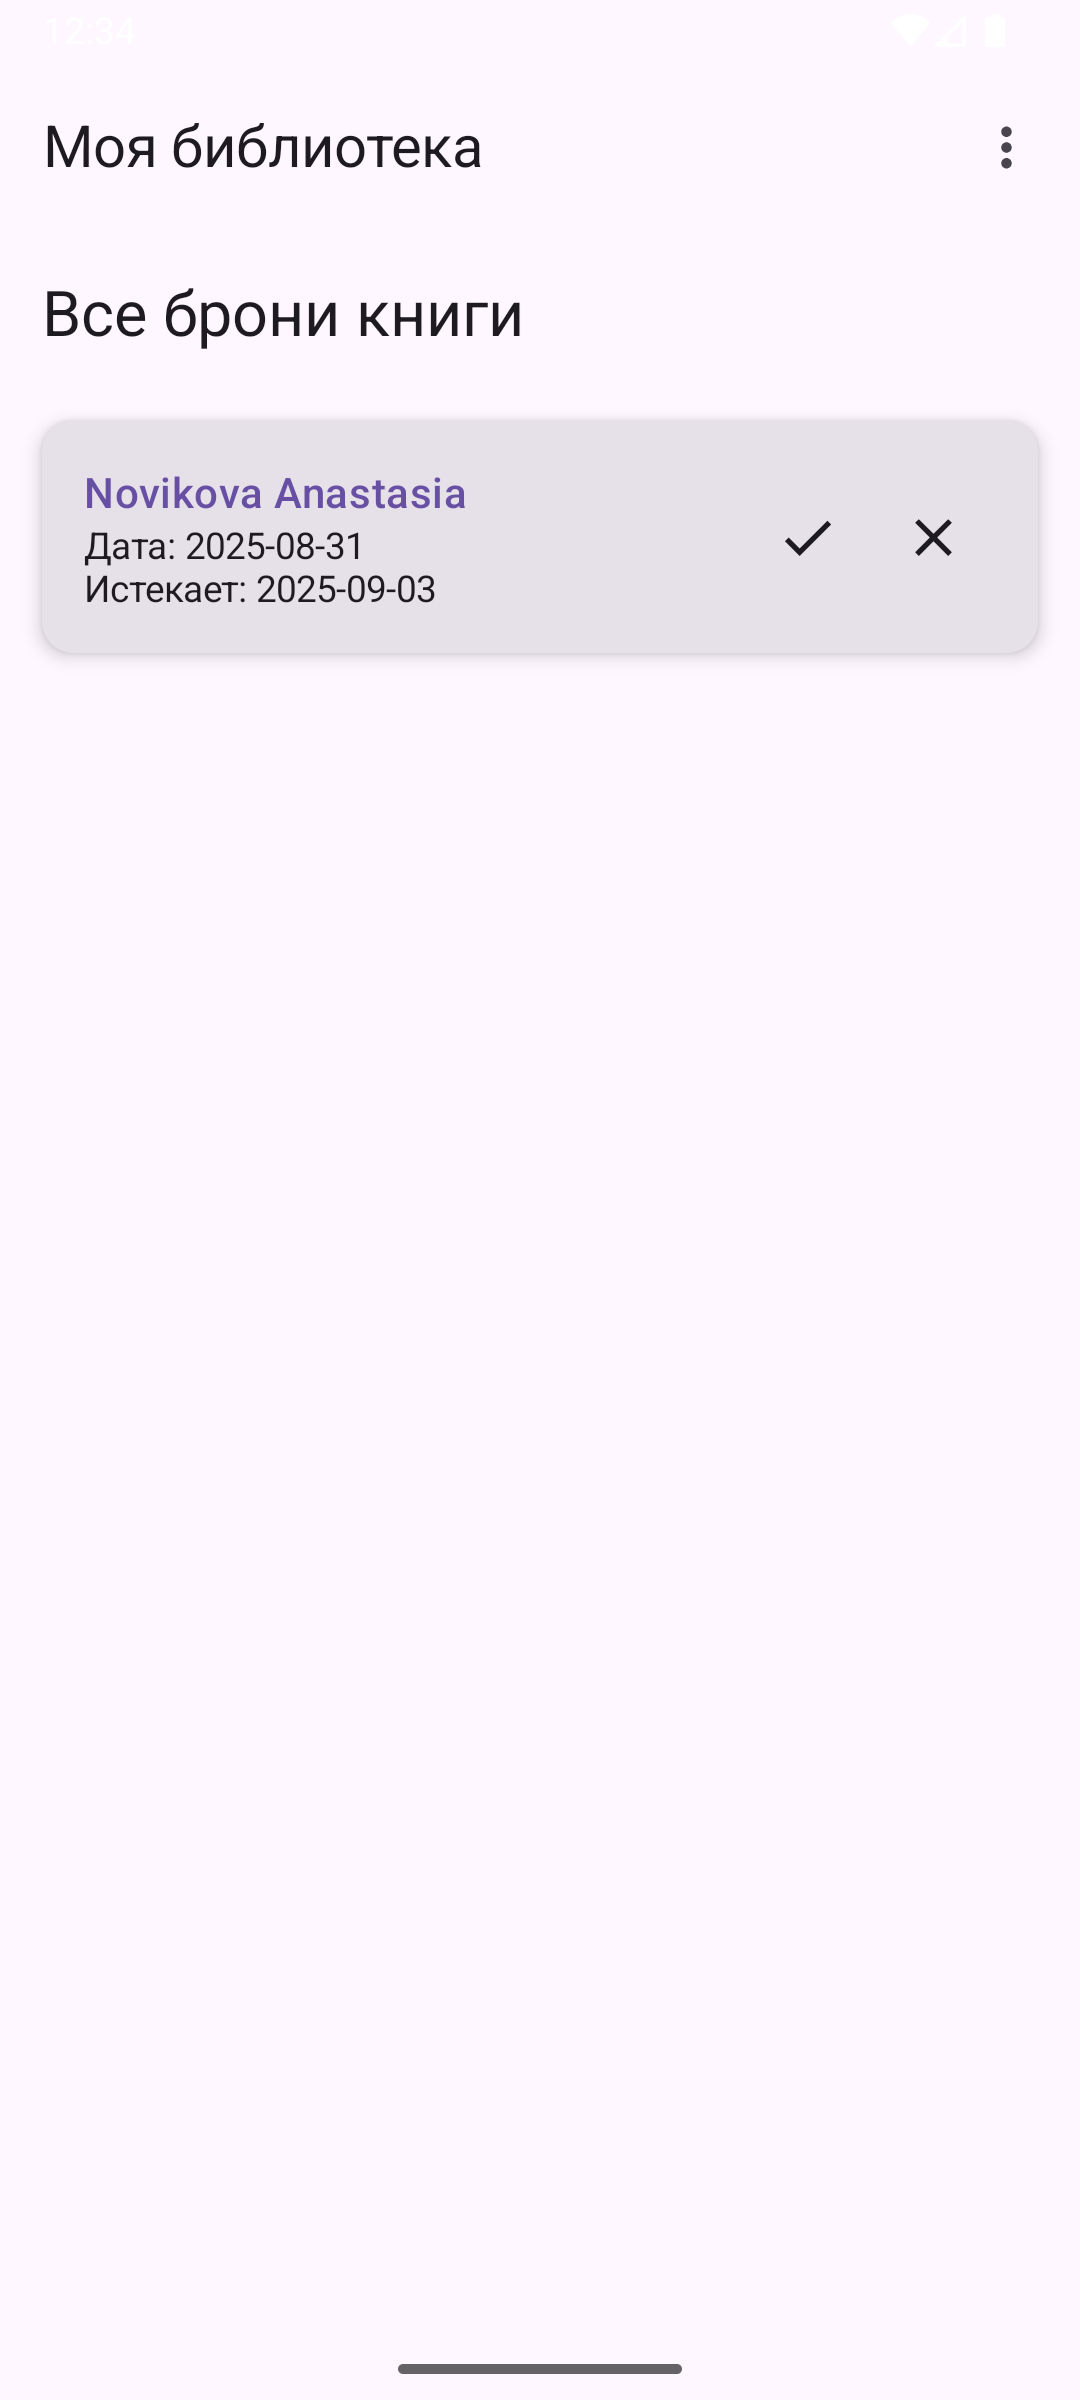
\includegraphics[scale=0.125]{img/reservation_list.png}
	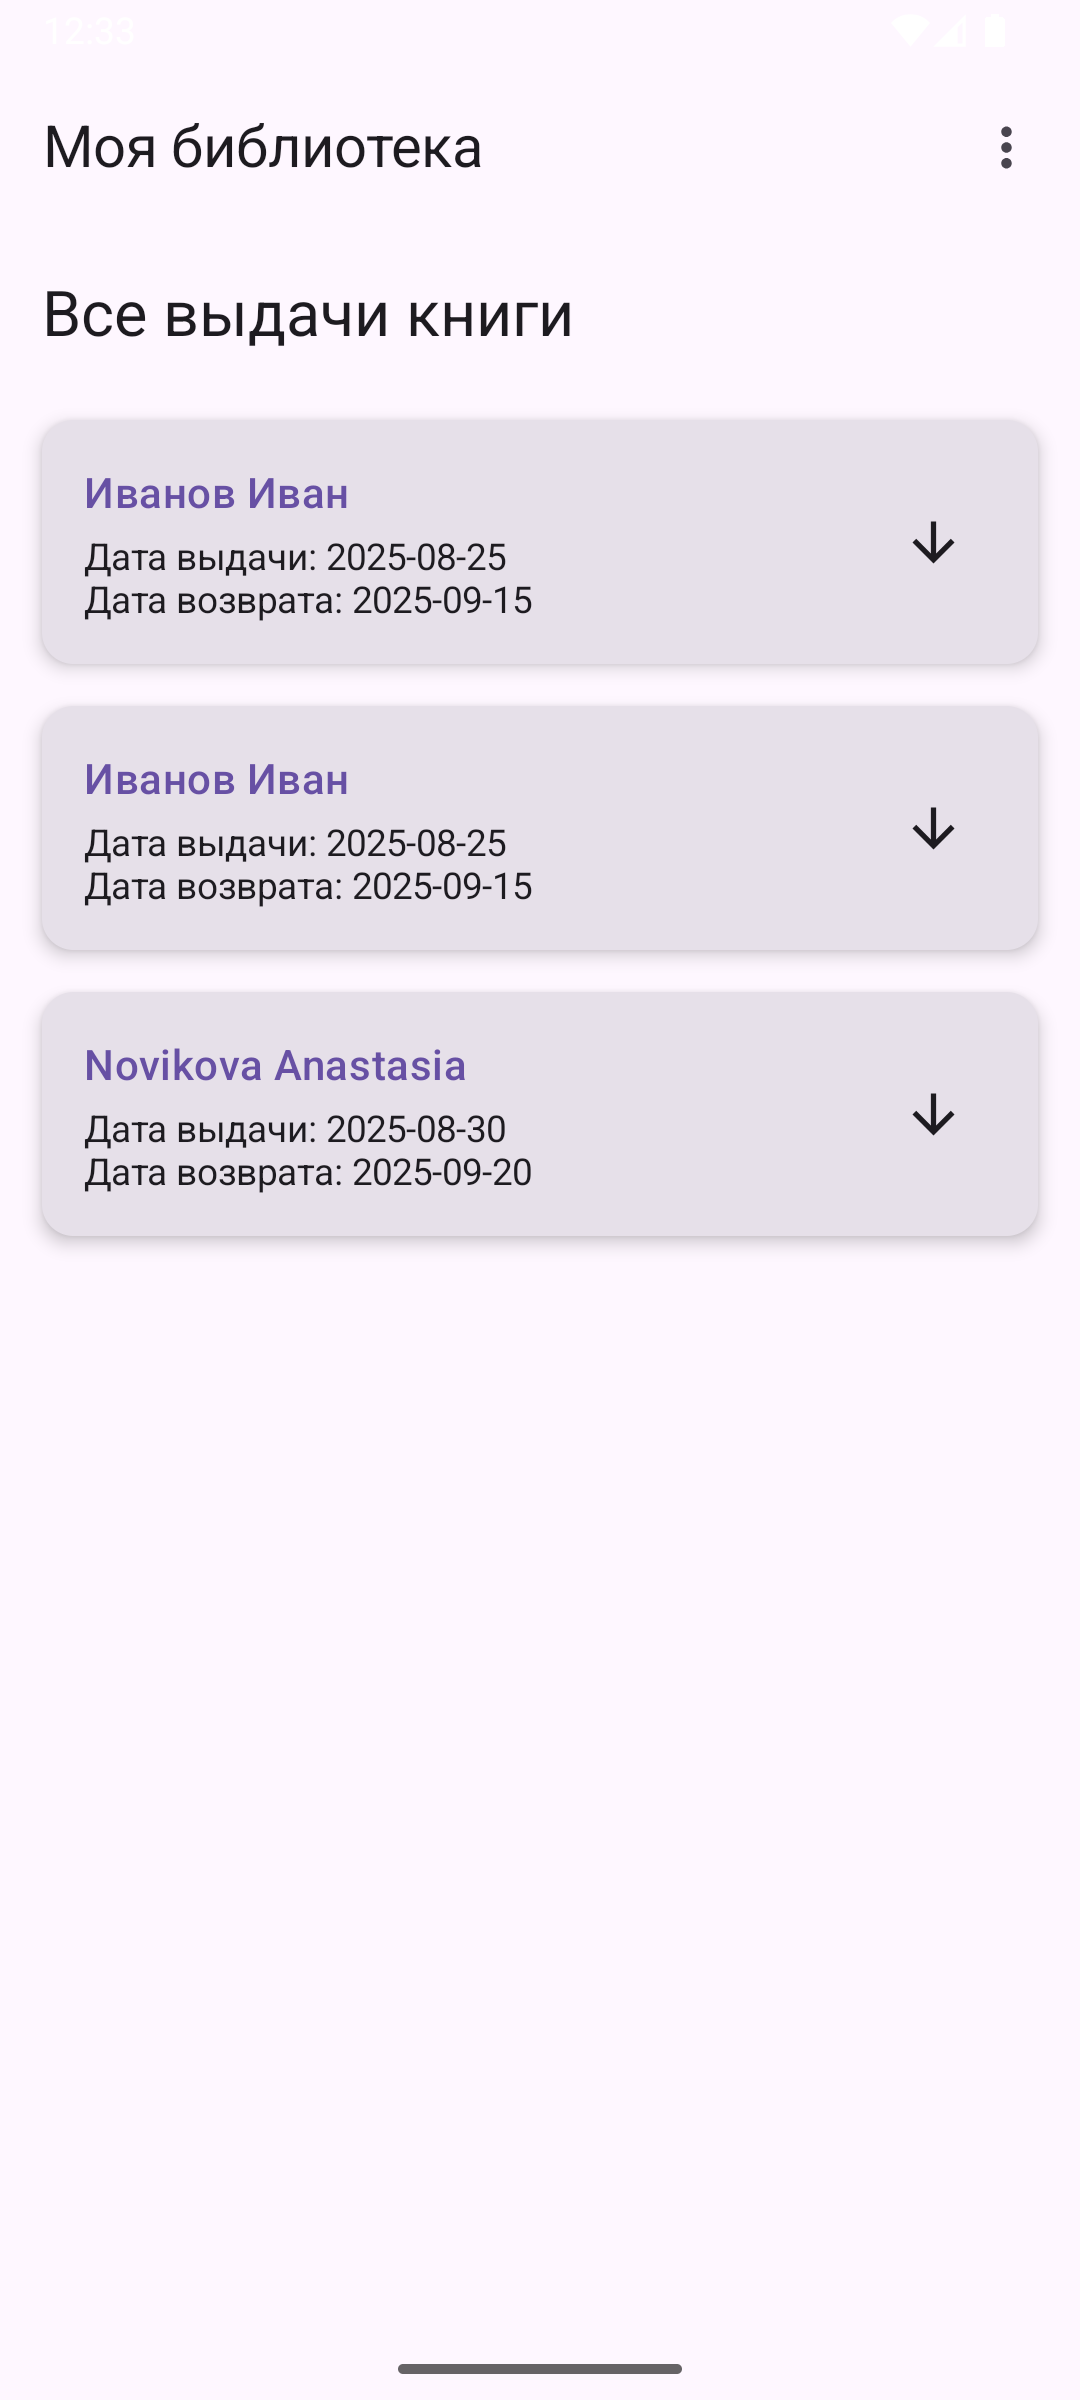
\includegraphics[scale=0.125]{img/issuance_list.png}
	\caption{Экраны библиотекаря}
\end{figure}

\begin{figure}[H]
	\centering
	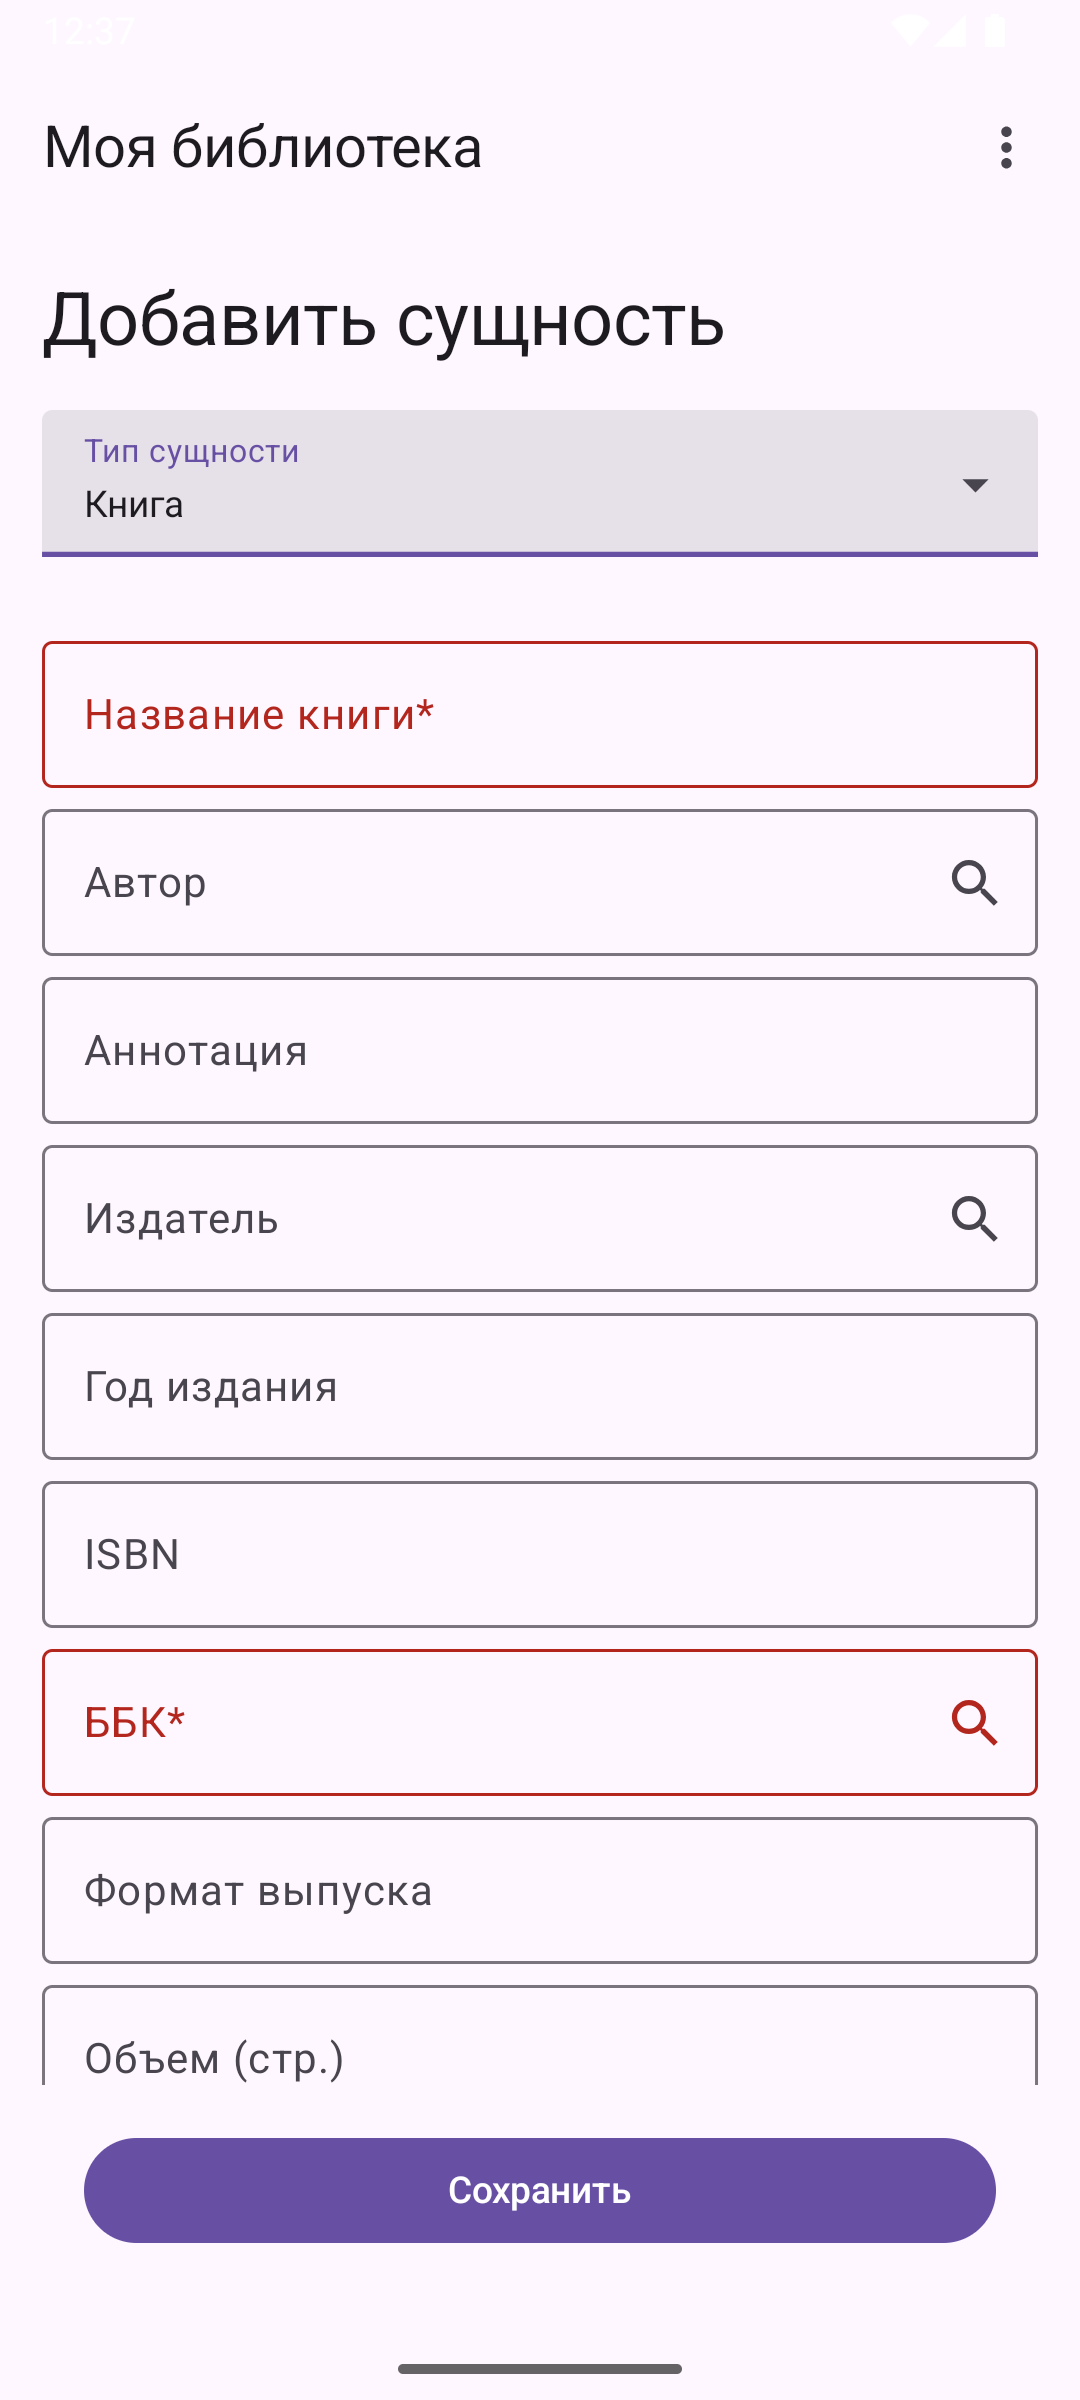
\includegraphics[scale=0.125]{img/book_add.png}
	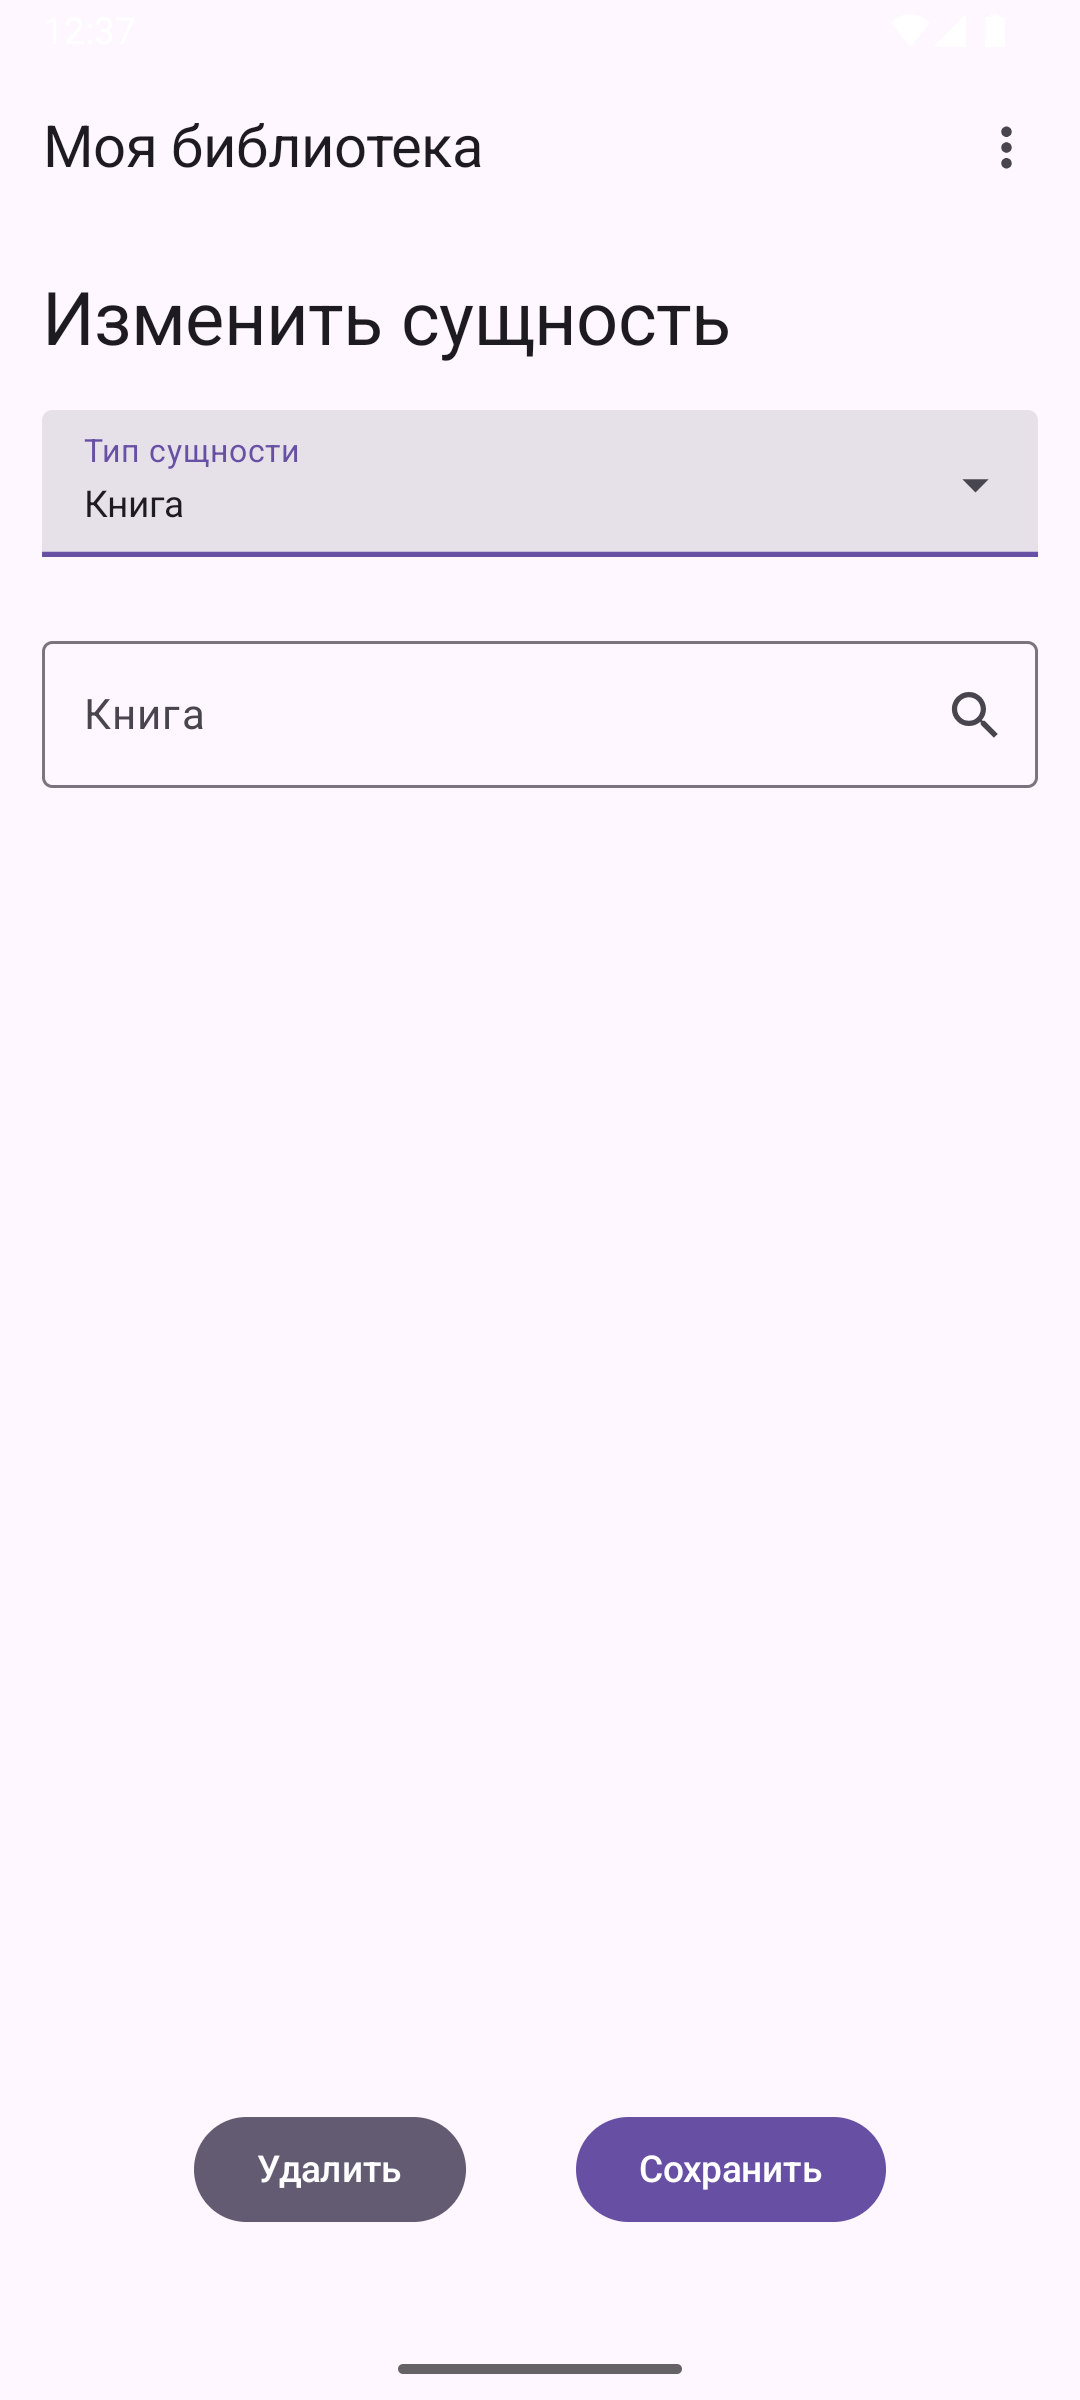
\includegraphics[scale=0.125]{img/book_edit_1.png}
	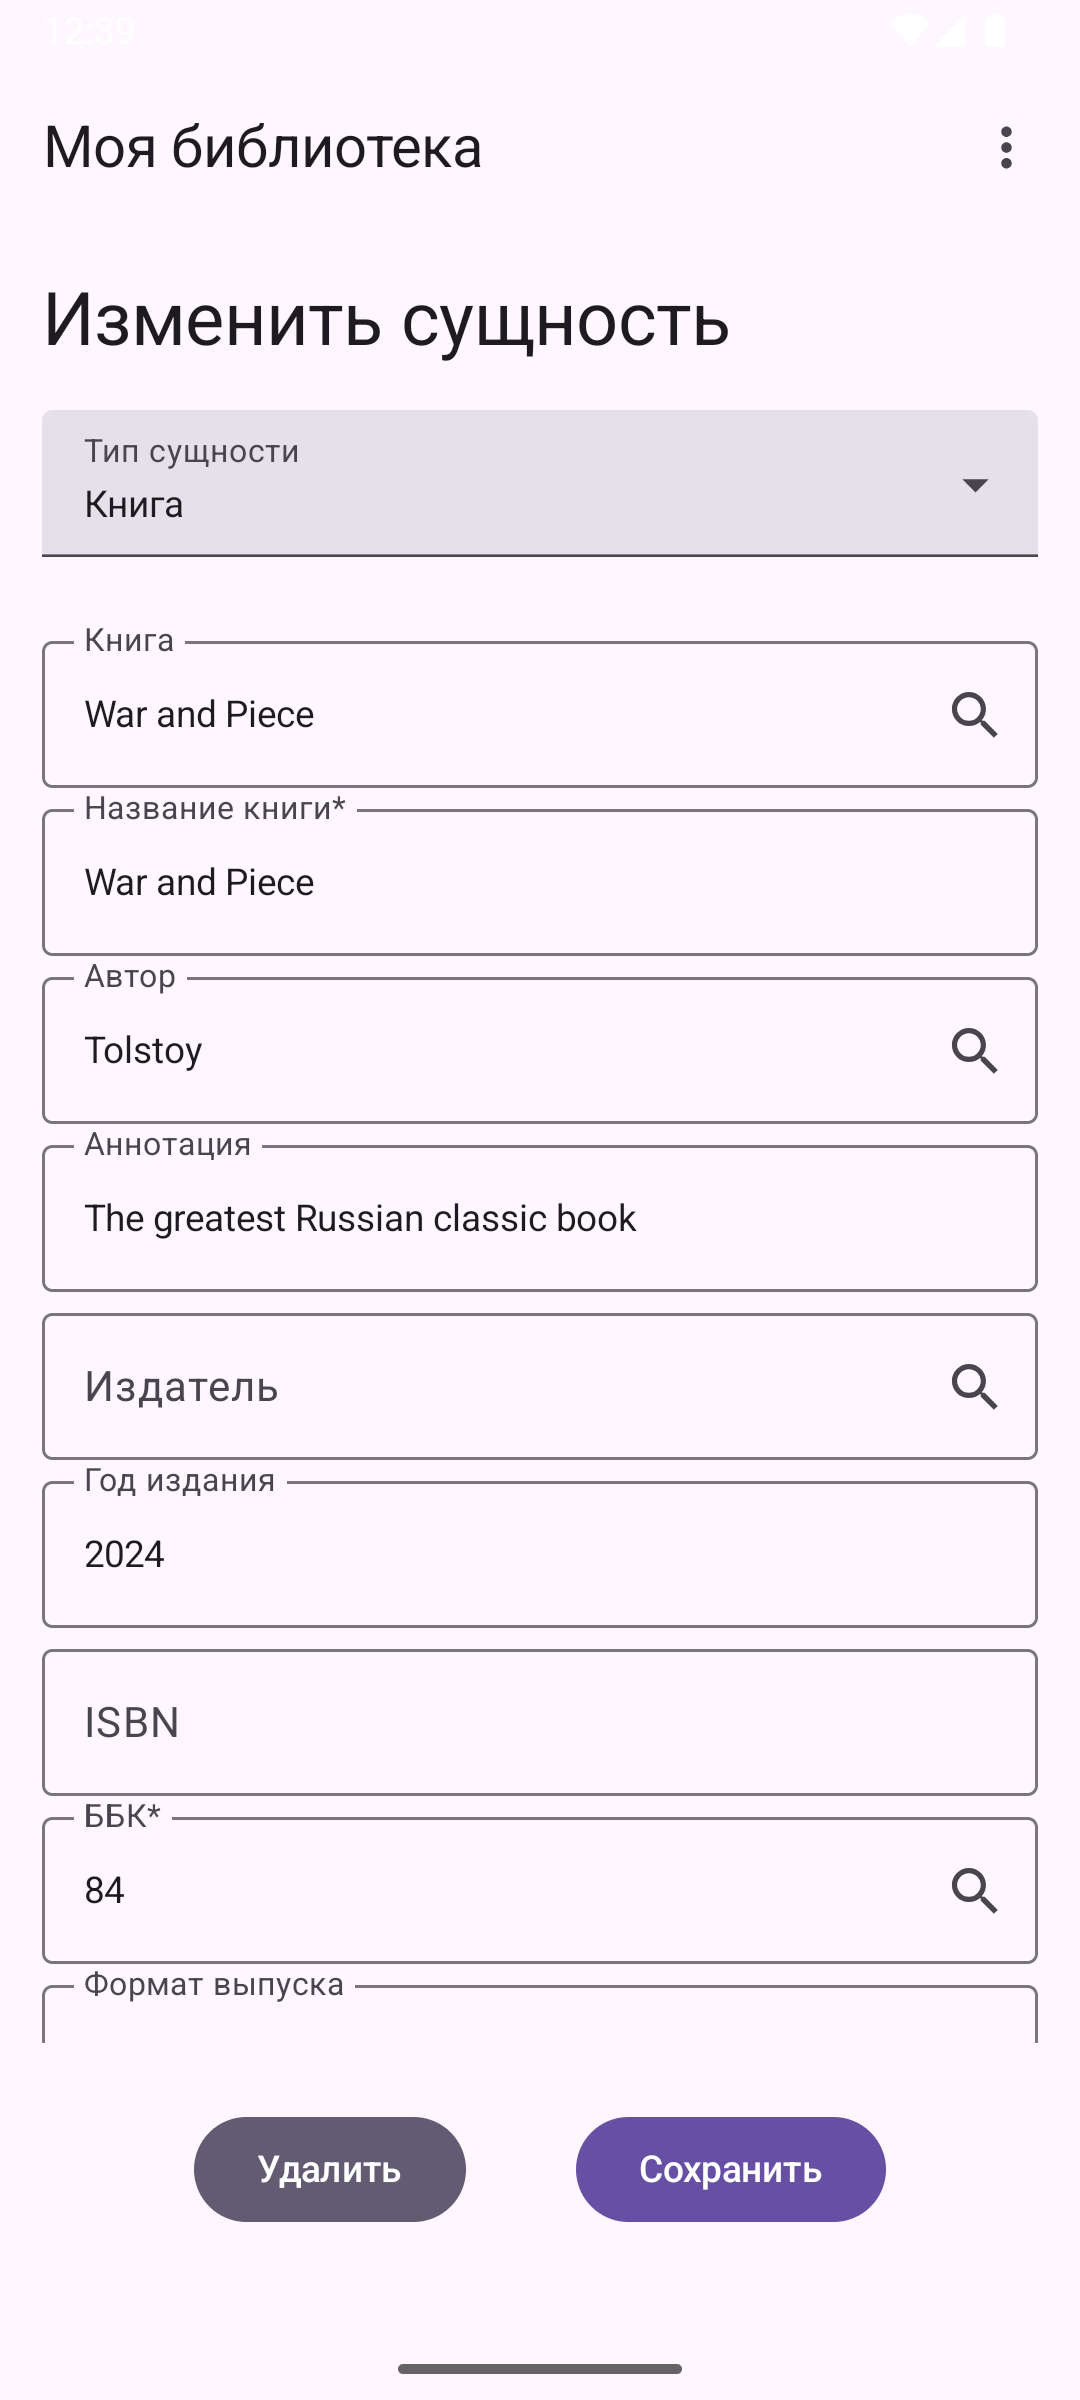
\includegraphics[scale=0.125]{img/book_edit_2.png}
	\caption{Экраны модератора}
	\label{fig:moderator}
\end{figure}

\clearpage

\textbf{ВЫВОД}

В данном разделе было проведено сравнение различных СУБД по выделенным критериям, описаны средства реализации ПО, представлено создание таблиц, функций, триггеров и ролей базы данных, а также продемонстрирована работа приложения.


\clearpage